
\newthought{Enigma Machines} and how the internal wiring of their rotors was reverse-engineered is the topic of this section. \index{Enigma}\index{permutation} We will follow a simplified version of Rejewski's description \cite{Rejewski1981} of his work.

An Enigma Machine applies a series of permutations to each typed letter, mapping it to another letter (which lights up on the Lampboard, see Figure \ref{fig:enigmaMachine}), thus encrypting a message\footnote{Enigma machines were used by the Nazis in WWII to encrypt/decrypt messages. The machines are rotor-based electromechanical typewriters. \url{http://en.wikipedia.org/wiki/Enigma_machine} has a detailed description of their internals.}.


\begin{marginfigure}[0.5in]
\begin{tikzpicture}[node distance=1.5cm]
\tikzstyle{perm} = [rectangle, rounded corners, minimum width=1cm, minimum height=1cm,text centered, draw=black]
\tikzstyle{arrow} = [thick,->,>=stealth]
\tikzstyle{rotor} = [dashed]

\node (lR) [perm] {$R$};

\node (lL) [perm, below of=lR, xshift=-2cm] {$L_k$};
\node (liL) [perm, below of=lR, xshift=2cm] {$L^{-1}_k$};

\node (lM) [perm, below of=lL] {$M_k$};
\node (liM) [perm, below of=liL] {$M^{-1}_k$};

\node (lN) [perm, below of=lM] {$N_k$};
\node (liN) [perm, below of=liM] {$N^{-1}_k$};

\node (lP) [perm, below of=lN] {$P$};
\node (liP) [perm, below of=liN] {$P^{-1}$};

\node (kb) [below of=lP] {Keyboard};
\node (lb) [below of=liP] {Lampboard};

\node [above of=lR, yshift=-0.7cm] {Reflector};

\draw [arrow] (lP) -- (lN);
\draw [arrow] (lN) -- (lM);
\draw [arrow] (lM) -- (lL);
\draw [arrow] (lL) to [out=90,in=180] (lR);
\draw [arrow] (lR) to [out=0,in=90] (liL);
\draw [arrow] (liL) -- (liM);
\draw [arrow] (liM) -- (liN);
\draw [arrow] (liN) -- (liP);
\draw [arrow] (kb) -- (lP);
\draw [arrow] (liP) -- (lb);

\draw [rotor] (lN) -- ($ (lN) + (2,0) $) node [above] {Right Rotor} -- (liN);
\draw [rotor] (lM) -- ($ (lM) + (2,0) $) node [above] {Middle Rotor} -- (liM);
\draw [rotor] (lL) -- ($ (lL) + (2,0) $) node [above] {Left Rotor} -- (liL);
\draw [rotor] (lP) -- ($ (lP) + (2,0) $) node [above] {Plugboard} -- (liP);

\end{tikzpicture}
\caption{Enigma Permutations}
\label{fig:enigmaMachine}
\end{marginfigure}

Electrical current flows from the typed letter through the plugboard, then the right rotor, the middle rotor and the left rotor. It then enters the reflector and goes back in reverse order through the same components ending up on the lampboard where the corresponding encrypted letter lights up. The plugboard, rotors and reflector have internal wirings which correspond to permutations in $S_{26}$\footnote{$S_{26}$ is the symmetric group of permutations of $\{1, 2, \ldots, 26\}$.}. The resulting permutation applied to a letter by the Enigma Machine is the product\footnote{We use the convention of permutation product as function composition, so for $A,B \in S_{26}$ we have $AB=A \circ B$ and $AB(x)=A(B(x))$.}:

$$
P^{-1} N_k^{-1} M_k^{-1} L_k^{-1} R L_k M_k N_k P
$$

The rotors rotate after each typed letter in the style of an odometer: the right rotor rotates one position after each typed letter, the middle rotor rotates one position after each full-circle rotation of the right rotor and the left rotor rotates one position after each full-circle rotation of the middle rotor. Rotating the rotors changes the permutations they will apply to a letter, so their permutations are indexed by $k$ in the product above and in the Figure \ref{fig:enigmaMachine}. We will see later how we can model these rotations with permutations.

The reflector pairs each letter with another (always different) letter, thus it is a product of 13 disjoint transpositions. A permutation made out of only disjoint transpositions is called a \textbf{proper involution}\index{involution}. We will see why the Enigma Machine designers chose a proper involution for the reflector. 

First though we need to collect some facts about permutations that we will use in our Enigma Machine analysis.

\begin{thm}\label{cycleDecomposition}
Every permutation can be written as a product of disjoint cycles. This product is unique (ignoring cycle order and order of elements in cycle).
\end{thm}

\begin{proof}
Let $\pi \in S_n$ be a permutation.

We start by choosing an arbitrary $x_1 \in \{1, \ldots, n\}$ and define for it the set 
$$
T_{x_1} = \{x_1, \pi(x_1), \pi^2(x_1), \ldots\}
$$

$\{1, \ldots, n\}$ is finite, $T_{x_1} \subseteq \{1, \ldots, n\}$, so $T_{x_1}$ is finite too. This means that sooner or later there exist $i < j$ with $\pi^j(x_1)=\pi^i(x_1)$ or $x_1=\pi^{j-i}(x_1)$. Then $ord(x_1)=j-i$ is the order of $x_1$. It follows that 

$$
T_{x_1} = \{x_1, \pi(x_1), \pi^2(x_1), \ldots, \pi^{ord(x_1)-1}(x_1)\}
$$

and $T_{x_1}$ implies the cycle $(x_1, \pi(x_1), \pi^2(x_1), \ldots, \pi^{ord(x_1)-1}(x_1))$. $T_{x_1}$ is called the $\pi$-orbit of $x_1$. Let's denote this cycle

$$
\langle x_1 \rangle = (x_1, \pi(x_1), \pi^2(x_1), \ldots, \pi^{ord(x_1)-1}(x_1))
$$

We now choose an arbitrary $x_2 \in \{1, \ldots, n\} \setminus T_{x_1}$. If there is no such $x_2$ we stop this process and jump to the  section in the proof after all $x_k$ have been chosen. We similarly define $T_{x_2}$ and cycle $\langle x_2 \rangle$.

$T_{x_2}$ and $T_{x_1}$ are disjoint\footnote{Assume $y \in T_{x_2} \cap T_{x_1}$. Then $y=\pi^i(x_1)$ and $y=\pi^j(x_2)$. It follows that $x_2 \in T_{x_1}$ or $x_1 \in T_{x_2}$, either one of which contradicts how $x_2$ was chosen. Another way to see this is by defining the following relationship: $\forall a, b \in S_n: a \sim b \equiv \exists n \in \mathbb{N}: b = \pi^n(a)$. It's not hard to see that $a \sim b$ so defined is an equivalence relationship and with it the $T_{x_i}$ become equivalence classes and partition $S_n$.}.

We continue and choose an arbitrary $x_3 \in \{1, \ldots, n\} \setminus (T_{x_1} \cup T_{x_2})$, and in general an arbitrary

$$
x_k \in \{1, \ldots, n\} \setminus (\bigcup^{k-1}_{i=1} T_{x_i})
$$

Since all the $T_{x_i}$ are non-empty and $\{1, \ldots, n\}$ is finite, we eventually have to stop. We then have chosen $x_1, x_2, \ldots, x_k$ and the corresponding sets $T_{x_1}, T_{x_2}, \ldots, T_{x_k}$ and cycles $\langle x_1 \rangle, \langle x_2 \rangle, \ldots, \langle x_k \rangle$.

The sets $T_{x_i}$ and their corresponding cycles are by construction pairwise disjoint. We also have $\{1, \ldots, n\} = \bigcup^{k}_{i=1} T_{x_i}$.

We define the permutation $\rho$ as the product of the cycles chosen above:

$$
\rho=\prod\limits^k_{i=1} \langle x_i \rangle
$$

and show that $\rho=\pi$. 

For all $y \in \{1, \ldots, n\}$ there exists a unique $1 \leq i \leq k$ such that $y \in T_{x_i}$.\footnote{Because $\{1, \ldots, n\} = \bigcup^{k}_{i=1} T_{x_i}$ and $T_{x_1}, T_{x_2}, \ldots, T_{x_k}$ are pairwise disjoint and form a partition of $\{1, \ldots, n\}$.}

So $y = \pi^j(x_i)$ for some index $0 \leq j < ord(x_i)$. Since the cycles are disjoint, only cycle $\langle x_i \rangle$ from $\rho$ affects $y$. We have

\begin{align*}
\rho(y) &= \langle x_i \rangle (y) \\
        &= \langle x_i \rangle (\pi^j(x_i)) \\
        &= \pi^{j+1}(x_i) \\
        &= \pi(\pi^j(x_i)) \\
        &= \pi(y)
\end{align*}

\end{proof}

Given two permutations $\pi, \rho \in S_n$, the product $\rho \pi \rho^{-1}$ is called a conjugate\index{conjugate} of $\pi$.

\begin{thm}\label{conjugationPreservesCycles}
Conjugation preserves cycle structure, i.e. conjugates have cycles of the same length with the same multiplicity.
\end{thm}

\marginnote{Incidentally Theorem \ref{conjugationPreservesCycles} is the reason why the products $\pi \rho$ and $\rho \pi$ have the same cycle structure. Even though in general $\pi \rho \neq \rho \pi$, $\pi \rho$ and $\rho \pi$ are conjugate. This was the question asked in Exercise 5.5 on page 34 from \bibentry{artin10}.}

\begin{proof}
Consider $\pi, \rho \in S_n$. From Theorem \ref{cycleDecomposition} we know that $\pi$ is a product of disjoint cycles $\pi = \prod^k_{i=1} \rho_i$. For the conjugate $\rho \pi \rho^{-1}$ we can write:

\begin{align*}
\rho \pi \rho^{-1} &= \rho \rho_1 \rho_2 \rho_3 \ldots \rho_k \rho^{-1} \\
&= \rho \rho_1 (\rho^{-1}\rho) \rho_2 (\rho^{-1} \ldots \rho) \rho_k \rho^{-1} \\
&= (\rho \rho_1 \rho^{-1}) (\rho \rho_2 \rho^{-1}) \ldots (\rho \rho_k \rho^{-1}) \\
&= \prod\limits^k_{i=1} \rho \rho_i \rho^{-1}
\end{align*}

so it is enough to prove the theorem for a cycle.

Let $\rho = (a_1, a_2, \ldots, a_r)$ be a cycle of length $r$. We have

$$
(\rho \rho \rho^{-1}) (\rho(a_i)) = (\rho \rho) (a_i) = \rho(a_{i+1}) 
$$

so $\rho \rho \rho^{-1}$ will have the cycle $(\rho(a_1), \rho(a_2), \ldots, \rho(a_r))$ with length $r$. Now assume that $x$ is moved by $\rho \rho \rho^{-1}$, so $(\rho \rho \rho^{-1})(x) \neq x$. It follows that $(\rho \rho^{-1})(x) \neq \rho^{-1} (x)$ or $\rho (\rho^{-1} (x)) \neq \rho^{-1} (x)$. This means that $\rho^{-1} (x) \in (a_1, a_2, \ldots, a_r)$ and $x \in (\rho(a_1), \rho(a_2), \ldots, \rho(a_r))$. It follows that $\rho \rho \rho^{-1} = (\rho(a_1), \rho(a_2), \ldots, \rho(a_r))$.

\end{proof}

\begin{marginfigure}[0.5in]
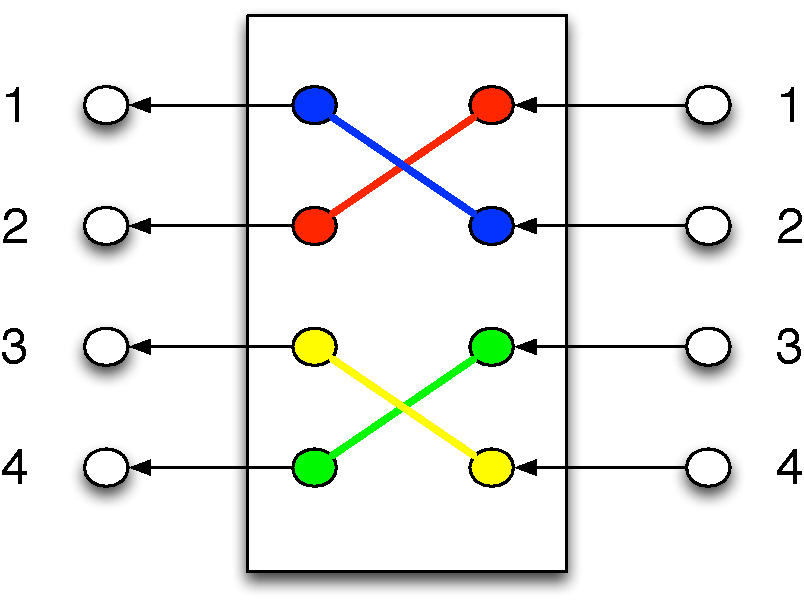
\includegraphics[scale=0.4]{rotorMotionBefore.pdf}
\caption{Initial Rotor}
\label{fig:rotorMotionBefore}
\end{marginfigure}

We have seen that an Enigma Machine permutation $E$ is the product
\begin{align*}
E &= P^{-1} N_k^{-1} M_k^{-1} L_k^{-1} R L_k M_k N_k P \\
  &= (L_k M_k N_k P)^{-1} R (L_k M_k N_k P) \\
  &= Q R Q^{-1}
\end{align*}

with $Q = (L_k M_k N_k P)^{-1}$. This means that $E$ is a conjugate of the reflector permutation $R$, and according to Theorem \ref{conjugationPreservesCycles} has the same cycle structure as $R$. So $E$ is a proper involution (because $R$ is) and also $E^{-1}=E$. The same Enigma Machine configuration was used to encrypt and decrypt a message, which was probably why the Enigma Machine designers chose a proper involution for $R$ and ultimately for $E$.

\begin{marginfigure}[0.5in]
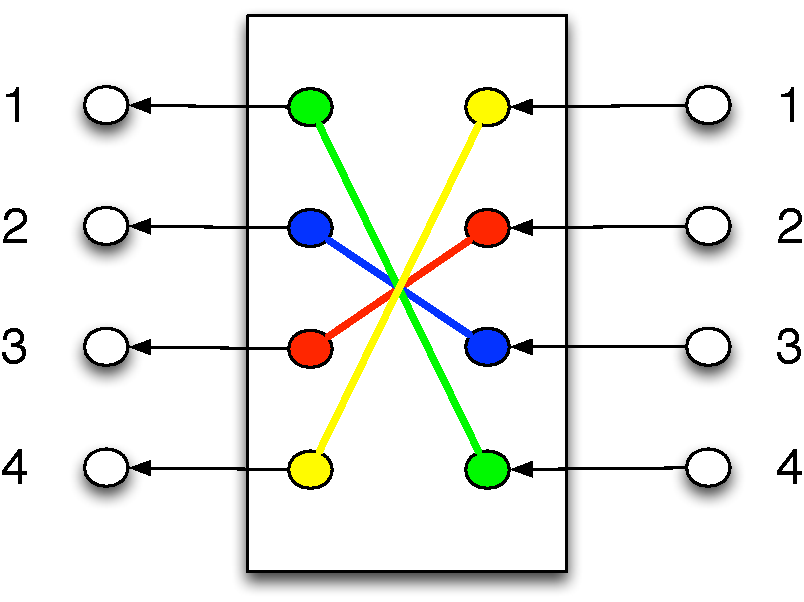
\includegraphics[scale=0.4]{rotorMotionAfter.pdf}
\caption{Rotor after one rotation}
\label{fig:rotorMotionAfter}
\end{marginfigure}

Let's analyse the rotor motion on the example in Figure \ref{fig:rotorMotionBefore}. It shows a small rotor with an internal wiring doing a permutation from $S_4$. It has $4$ inputs/outputs and permutation $\pmt{(12)(34)}$. Rotating it down one position as in Figure \ref{fig:rotorMotionAfter} doesn't change its internal wiring but shifts the inputs/outputs. Input one is now connected to the yellow wire instead of the red, input two to the red wire instead of the blue, etc. The resulting permutation is $\pmt{(14)(23)}$. The inputs have been shifted according to $(4321)$ and the outputs according to $\pmt{(1234)}$, so $\pmt{(14)(23)}=\pmt{(1234)} \pmt{(12)(34)}  \pmt{(4321)}$. In general one rotation of a rotor is equivalent to conjugating it with the full cycle permutation $\sigma$, in other words we have $N_{k+1}=\sigma N_k \sigma^{-1}$. To see why this is true, consider input $x$ touches the red wire in the rotor after the rotation. We don't know yet where the rotor will map $x$. We do know that if $x$ touches the red wire in the rotor after the rotation, then $\sigma^{-1}(x)$ is touching the red wire before the rotation (because all inputs and outputs have been shifted down). Also we know where the rotor maps any input $y$ before the rotation, namely to $N_k(y)$. So $\sigma^{-1}(x)$ is mapped to $N_k(\sigma^{-1}(x))$. And any output from before the rotation is shifted down once after the rotation, in this case to $\sigma(N_k(\sigma^{-1}(x)))$ after the rotation. Collecting this tracing into one expression, we have $N_{k+1}(x) = \sigma(N_k(\sigma^{-1}(x)))$.

Assuming only the right rotor moves, the first six Enigma permutations are:

\begin{equation} \label{sixEnigma1}
\begin{split}
A &= P^{-1} N_0^{-1} M_0^{-1} L_0^{-1} R L_0 M_0 N_0 P \\
B &= P^{-1} \sigma N_0^{-1} \sigma^{-1} M_0^{-1} L_0^{-1} R L_0 M_0 \sigma N_0 \sigma^{-1} P \\
C &= P^{-1} \sigma^{2} N_0^{-1} \sigma^{-2} M_0^{-1} L_0^{-1} R L_0 M_0 \sigma^{2} N_0 \sigma^{-2} P \\
D &= P^{-1} \sigma^{3} N_0^{-1} \sigma^{-3} M_0^{-1} L_0^{-1} R L_0 M_0 \sigma^{3} N_0 \sigma^{-3} P \\
E &= P^{-1} \sigma^{4} N_0^{-1} \sigma^{-4} M_0^{-1} L_0^{-1} R L_0 M_0 \sigma^{4} N_0 \sigma^{-4} P \\
F &= P^{-1} \sigma^{5} N_0^{-1} \sigma^{-5} M_0^{-1} L_0^{-1} R L_0 M_0 \sigma^{5} N_0 \sigma^{-5} P 
\end{split}
\end{equation}

\begin{marginfigure}[1.0in]
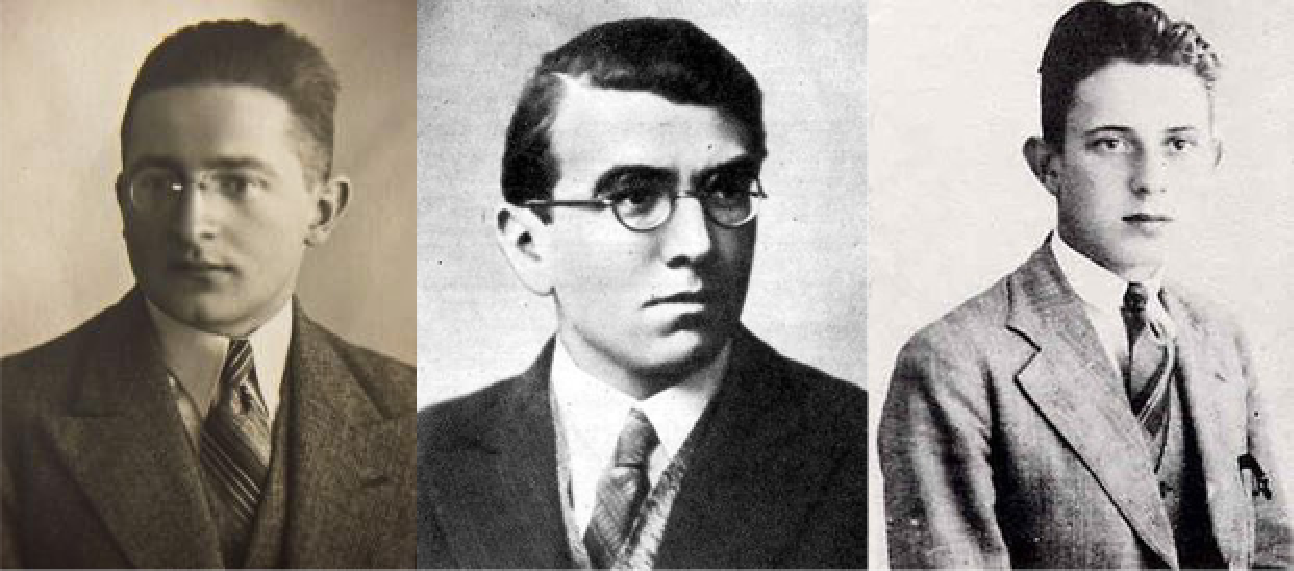
\includegraphics[scale=0.25]{attackers.pdf}
\end{marginfigure}

The first six permutations are important because of how the German Nazis chose to operate Enigma. It was known to the code breakers\footnote{Marian Rejewski, Henryk Zygalski and Jerzy Różycki. \url{http://en.wikipedia.org/wiki/Marian_Rejewski}} that after configuring Enigma to its daily settings and before sending a message, an operator would send a block of three letters twice. The three letters encoded a message key and because transmission lines were deemed unreliable, these three letters would be sent twice. This means that for each message transmission the input to permutations $A$ and $D$ was the same letter (similar for $B$ and $E$ and for $C$ and $F$). The code breakers had access to two months of intercepted messages and daily key settings. So they could determine that an unknown letter $u$ was mapped by $A$ to the observed letter $x$ and by $D$ to the observed letter $y$, so $A(u)=x$ and $D(u)=y$. Because $A$ and $D$ are each proper involutions\footnote{This is one example of why choosing a proper involution as the encryption permutation was a bad idea for Enigma Machines. As it turns out it was fatally bad: It was the main weakness that allowed the British \textit{bombe machine} built at Bletchley Park by Alan Turing and Gordon Welchman to decrypt Enigma encrypted messages. \url{http://en.wikipedia.org/wiki/Cryptanalysis_of_the_Enigma\#British_bombe}} it also holds that $A(x)=u$ and $D(y)=u$. It follows that $AD(y)=A(D(y))=A(u)=x$. So $AD$ maps one observed letter to another observed letter. With enough messages in a given day, each letter of the alphabet will be observed which then completely defines $AD$ and similarly $BE$ and $CF$. So for a given day $AD$, $BE$ and $CF$ were known permutations. The goal now is to factor $AD$ into $A$ and $D$. 

We need a way to compute how many possible factorizations there are and a way to generate all possibilities. To accomplish this we need to collect some properties of products of proper involutions. We will use a simplified approach similar to the approach described in chapter 3.8 of \citet{lawrence2021introduction}\footnote{\cite{lawrence2021introduction}}.

\begin{thm}\label{involutionproduct}
Let $\pi = \tau \rho$ be the product of proper involutions $\tau$ and $\rho$ and let $x \in \{1, \ldots, n\}$. Then the $\pi$-orbits of $x$ and $\rho(x)$ are disjoint and have equal length.
\end{thm}

\begin{proof}

Reminder here that the $\pi$-orbit of $x$ is 

$$
T_x = \{x, \pi(x), \pi^2(x), \ldots, \pi^{ord(x)-1}(x)\}
$$

Assume the two orbits are not disjoint and $y \in T_x \cap T_{\rho(x)}$. For some integers $i$ and $j$ we have $y = \pi^i(x) = \pi^j(\rho(x))$. Let $m = ord(\rho(x))$ and let $(k - 1) m < j \leq k m$ for some $k$. Then 

$$
\pi^{i + k m - j} (x) = \pi^{k m} (\rho(x)) = \rho(x)
$$

Let $n = i + k m - j$ and so

$$
\rho (\pi^n (x)) = \rho^2(x) = x
$$

because $\rho$ is a proper involution (so it is its own inverse).

We now have two cases: $n$ can be even or odd.

When $n = 2 l$:
\begin{align*}
\rho \pi^n &= \rho \pi^l \pi^l \\
           &= \rho \underbrace{(\tau\rho) (\tau\rho) \ldots (\tau\rho)}_{l\text{-times}}  \pi^l \\
           &= \underbrace{(\rho \tau) (\rho \tau) \ldots (\rho \tau)}_{l\text{-times}} \rho \pi^l \\
           &= \pi^{-l} \rho \pi^l
\end{align*}

This means that $\rho \pi^n$ is a conjugate of $\rho$ and thus it is a proper involution and cannot have $x$ mapping to itself. We have a contradiction.

When $n = 2 l + 1$:

\begin{align*}
\rho \pi^n &= \rho \pi^l \tau \rho \pi^l \\
           &= \rho \underbrace{(\tau\rho) (\tau\rho) \ldots (\tau\rho)}_{l\text{-times}}  \tau \rho \pi^l \\
           &= \underbrace{(\rho \tau) (\rho \tau) \ldots (\rho \tau)}_{l\text{-times}} \rho \tau \rho \pi^l \\
           &= (\rho \pi)^{-1} \tau (\rho \pi^l)
\end{align*}

This means that $\rho \pi^n$ is a conjugate of $\tau$ and thus it is a proper involution and cannot have $x$ mapping to itself. Again we have a contradiction.

We just showed that the $\pi$-orbits of $x$ and $\rho(x)$ are disjoint. To show that the orbits have the same length, we again reach for this useful identity: for any integer $m$ we have $\rho \pi^m = \pi^{-m} \rho$. This is because

\begin{align*}
\rho \pi^m &= \rho \underbrace{(\tau\rho) (\tau\rho) \ldots (\tau\rho)}_{m\text{-times}} \\
           &= \underbrace{(\rho \tau) (\rho \tau) \ldots (\rho \tau)}_{m\text{-times}} \rho \\
           &= \pi^{-m} \rho
\end{align*}

The identity allows for this equivalence: 

$$
\pi^{-m}(\rho(x)) = \rho(x) \Leftrightarrow \rho(x) = \rho(\pi^m(x)) \Leftrightarrow \pi^m(x) = x
$$

It means that the $\pi^{-1}$-orbit of $\rho(x)$ has the same length as the $\pi$-orbit of $x$. But $\pi^{-1}$-orbit and $\pi$-orbit of an element are the same\footnote{Just walk the cycle backwards.}.
So the $\pi$-orbits of $x$ and $\rho(x)$ have the same length.
\end{proof}

\begin{thm}\label{involutionproduct2}
Let $\pi = \tau \rho$ be the product of proper involutions $\tau$ and $\rho$ and let $x \in \{1, \ldots, n\}$. Then the $\pi$-orbits of $\tau(x)$ and $\rho(x)$ are equal. In addition to that, the $\pi$-orbit of $x$ is mapped by $\tau$ and $\rho$ onto this common $\pi$-orbit of $\tau(x)$ and $\rho(x)$.
\end{thm}

\begin{proof}

Keeping in mind that a proper inversion is its own inverse, we have:

\begin{align*}
\rho(x) &= \rho(x) \\
        &= \rho(\tau^2(x)) \\
        &= (\rho \tau) (\tau(x)) \\
        &= \pi^{-1} (\tau(x))
\end{align*}

so then $\pi(\rho(x)) = \tau(x)$ and $\tau(x)$ is in the $\pi$-orbit of $\rho(x)$.

Using the $\rho \pi^m = \pi^{-m} \rho$ identity again, we see that

$$
\rho (\pi^m (x)) = \pi^{-m}(\rho(x))
$$

so $\rho$ maps the $\pi$-orbit of $x$ onto the $\pi$-orbit of $\rho(x)$. 

To see where $\tau$ maps the $\pi$-orbit of $x$ we need a similar identity, so lets deduce it:

\begin{align*}
\tau \pi^m &= \tau \underbrace{(\tau\rho) (\tau\rho) \ldots (\tau\rho)}_{m\text{-times}} \\
           &= \tau \tau \underbrace{(\rho\tau) (\rho\tau) \ldots (\rho\tau)}_{m-1\text{-times}} \rho \\
           &= \pi^{-m+1} \rho \\
           &= \pi^{-m+1} \pi^{-1} \tau \\
           &= \pi^{-m} \tau
\end{align*}


We can use this identity for:

\begin{align*}
\tau(\pi^m(x)) &= \pi^{-m}(\tau(x)) \\
               &= \pi^{-m}(\pi\rho)(x) \\
               &= \pi^{1-m} (\rho(x)) 
\end{align*}

so $\tau$ also maps the $\pi$-orbit of $x$ onto the $\pi$-orbit of $\rho(x)$. 

\end{proof}

\begin{thm}\label{involutionproduct3}
Let $\pi = \tau \rho$ be the product of proper involutions $\tau$ and $\rho$ and let $x \in \{1, \ldots, n\}$. Let $y \notin T_x \cup T_{\rho(x)}$. Then $\rho(y) \notin T_x \cup T_{\rho(x)}$.
\end{thm}

\begin{proof}

Assume $\rho(y) \in T_x \cup T_{\rho(x)}$. Two cases:

First case: $\rho(y) \in T_x$. Then $\rho(y) = \pi^m(x)$ for some $m \in \mathbb{N}$. Keeping in mind again that the a proper involution is its own inverse, we apply $\rho$ to both sides to get

$$
y = (\rho \pi^m)(x) = \pi^{-m} (\rho(x))
$$

so $y \in T_{\rho(x)}$ which is a contradiction.

Second case: $\rho(y) \in T_{\rho(x)}$. We proceed similarly:

$\rho(y) = \pi^m(\rho(x))$ for some $m \in \mathbb{N}$ so

$$
y = (\rho \pi^m)(\rho(x)) = \pi^{-m} (\rho \rho)(x) = \pi^{-m} (x)
$$

so $y \in T_x$ which is a contradiction.

\end{proof}


\begin{thm}\label{involutionproduct4}
Let $\pi = \tau \rho$ be the product of proper involutions $\tau$ and $\rho$. Then the cycle lengths of $\pi$ that are greater than one come in even numbers.
\end{thm}

\begin{proof}

Let $(a b)$ be a cycle of $\tau$. We have two cases: 

Case 1: $(a b)$ is also a cycle of $\rho$. Then the product $\pi$ has cycles $(a)$ and $(b)$ of length one.

Case 2: $(a b)$ is not a cycle of $\rho$. Then it must have a cycle $(a c_{1})$ for some $c_{1}$. In $\tau$ there must be a cycle $(c_{1} c_{2})$ for some $c_{2}$. In $\rho$ again there must be a cycle $(c_{2} c_{3})$ for some $c_{3}$, $\ldots$ (remember, $\rho$ and $\tau$ are proper involutions, so each element participates in one and only one 2-cycle). We stop with a cycle $(c_{2k} b)$ in $\rho$, which eventually must happen. Then the product $\pi$ has cycles $(c_{2k} c_{2k - 2} \ldots c_{2} a)$ and $(c_{1} c_{3} c_{2k-1} b)$ of length $k$.

\end{proof}

We are ready to tackle the factorization. To recap, we have a permutation $\pi$ that we know and we also know it is a product of two proper involutions. Our goal is to find out how many possible factorizations into two proper involutions there are and how do we generate all the factorizations (because we need the factors to determine the first rotor wiring).

\begin{thm}\label{involutionproduct5}
Let $\pi \in S_{2n}$ be a permutation composed of just two disjoint cycles of length $n$. Then $\pi$ has exactly $n$ factorizations into two proper involutions.
\end{thm}

\begin{proof}

Pick an $a \in \{1, \ldots, 2n\}$. It is part of one of the two cycles. We are looking for possible $\pi = \tau \rho$ factorizations, with both $\tau$ and $\rho$ being proper involutions.
The two $\pi$-orbits of the two cycles are $A := T_a = \{a, \pi(a), \ldots, \pi^{n-1}(a)\}$ and $B := S_{2n} \setminus A$.

We are going to construct all the possible $\rho$ using the previous theorems as constraints (once a possible $\rho$ is constructed, it also fully determines the other factor, $\tau$). 

For example, because of theorem \ref{involutionproduct} we have to pick some element from $B$ for $\rho(a)$: $\rho(a) \in B$. We will argue that once this choice has been made, the complete factorization has been determined. Let's see why. What value should $\rho(\pi(a))$ take ? Again, using the identity $\rho \pi^m = \pi^{-m} \rho$, we get $\rho(\pi(a)) = \pi^{-1}(\rho(a))$. By repeatedly using the identity as we move $\pi$-forward in the cycle with $a$, we move $\pi$-backwards in the other cycle and at each stop we make another pair for the proper involution $\rho$. 

\begin{figure}
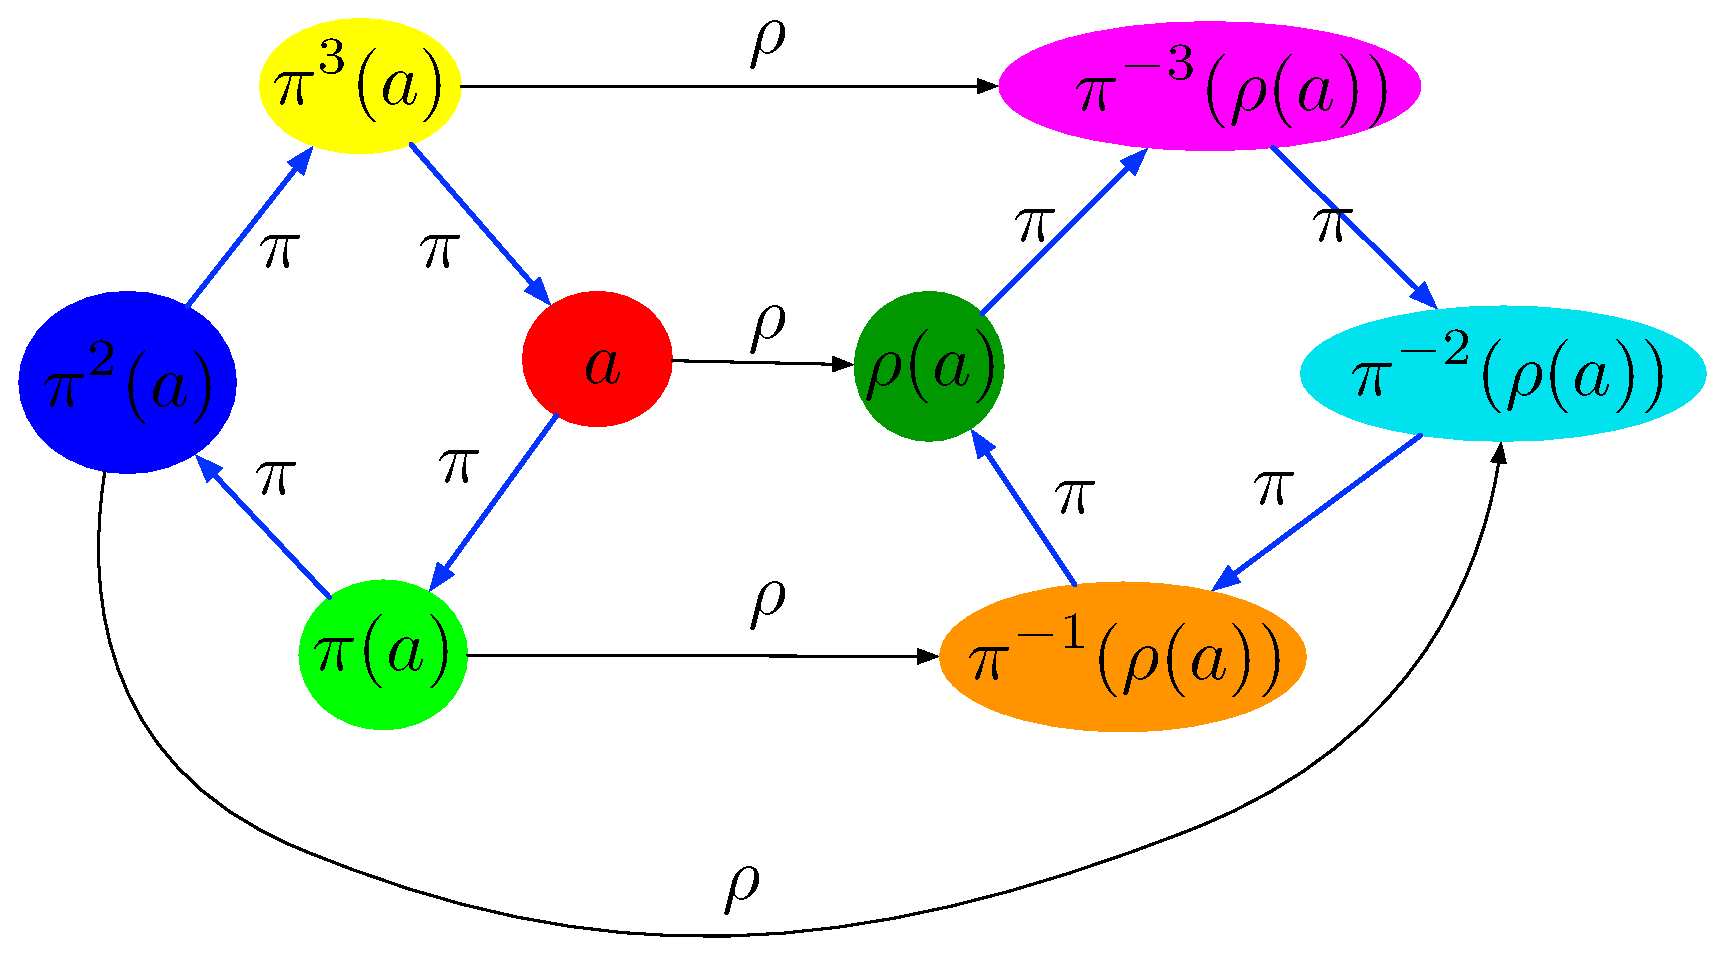
\includegraphics[scale=0.35]{enigma1.pdf}
\caption{Constructing $\rho$.}
\label{rhoconstructionexample}
\end{figure}

Figure \ref{rhoconstructionexample} shows the process for an example with two cycles of length four. After setting an $a$ and picking where to map $\rho(a)$, everything else is determined (the labels in the figure show the expressions determining the relationships).

There are $n$ ways to pick an element from $B$, hence we can construct $n$ different $\rho$, so $n$ different factorizations $\pi = \tau \rho$. It doesn't matter which $a$ we start with. Through the cycle-wise rotation in cycle with $a$ and counter-cycle rotation in the cycle with $\rho(a)$, we see all $n$ possible $\rho$ constructions, regardless which $a$ is our anchor. Does it matter from which cycle we choose the anchor ? It doesn't because again the same factorizations would be produced if all the $\rho$-arrows in figure \ref{rhoconstructionexample} were reversed.

\end{proof}

Now theorem \ref{involutionproduct4} assures us that any product of two proper involutions has cycle lengths greater than one occurring an even number of times. We can always pair up two cycles of the same length. Theorems \ref{involutionproduct2} and \ref{involutionproduct3} help us isolate the pairings and construct the factors by restricting ourselves to each pairing and using the construction from theorem \ref{involutionproduct5} to build the possible factors for each paired restriction. We multiply all the restricted $\tau$'s to get the unrestricted $\tau$ and multiply all the restricted $\rho$'s to get the unrestricted $\rho$.

So how many factorizations are there for a given product $\pi$? Lets say $\pi$ has $2m_k$ cycles of length $k$. In how many ways can we pair up these $2m_k$ cycles? 

\begin{thm}\label{numpairings}
The number of ways $W$ to form $m$ pairs from the integers \\
$\{1, 2, \ldots, 2m\}$ is

$$
W = \frac{(2m)!}{2^m m!}
$$

\end{thm}

\begin{proof}

Integer one can be paired with $2m-1$ other integers. Picking an unpaired remaining integer, it can be paired with $2m-3$ other integers, etc.

It follows that

\begin{align*}
W &= (2n-1)(2n-3) \ldots 5 \cdot 3 \cdot 1 \\
  &= (2n-1)(2n-3) \ldots 5 \cdot 3 \cdot 1 \cdot \frac{(2m)(2n-2)(2n-4) \ldots 4 \cdot 2}{(2m)(2n-2)(2n-4) \ldots 4 \cdot 2} \\
  &= \frac{(2m)!}{(2m)(2n-2)(2n-4) \ldots 4 \cdot 2} \\
  &=\frac{(2m)!}{2^m m!}
\end{align*}

\end{proof}

Which means that if $\pi$ has $2m_k$ cycles of length $k$, we can produce 

$$
\frac{k^{m_k} (2m_k)!}{2^{m_k} m_k!}
$$

factorizations restricted to those cycles. Multiplying over all the possibly cycle lengths greater than one gives us the number of factorizations

$$
\prod_{k \text{ cycle length}}\frac{k^{m_k} (2m_k)!}{2^{m_k} m_k!}
$$

We return to the first six Enigma permutations \ref{sixEnigma1}. After using the factorization to factor $AD$, $BE$ and $CF$, we know possible solutions for $A$, $B$, $C$, $D$, $E$ and $F$. The plugboard settings $P$ were found out from French spies, $\sigma$ is the full cycle permutation. We can drop the subscripts from $M$ and $L$ because we assume they don't rotate for the first six typed letters and from $N$ because we know how to express its rotations. We get:

\begin{equation} \label{sixEnigma2}
\begin{split}
A &= P^{-1} N^{-1} M^{-1} L^{-1} R L M N P \\
B &= P^{-1} \sigma^{-1} N^{-1} \sigma M^{-1} L^{-1} R L M \sigma^{-1} N \sigma P \\
C &= P^{-1} \sigma^{-2} N^{-1} \sigma^{2} M^{-1} L^{-1} R L M \sigma^{-2} N \sigma^{2} P \\
D &= P^{-1} \sigma^{-3} N^{-1} \sigma^{3} M^{-1} L^{-1} R L M \sigma^{-3} N \sigma^{3} P \\
E &= P^{-1} \sigma^{-4} N^{-1} \sigma^{4} M^{-1} L^{-1} R L M \sigma^{-4} N \sigma^{4} P \\
F &= P^{-1} \sigma^{-5} N^{-1} \sigma^{5} M^{-1} L^{-1} R L M \sigma^{-5} N \sigma^{5} P 
\end{split}
\end{equation}

The unknowns in equations \ref{sixEnigma2} are $M$, $L$, $R$ and $N$. Our goal is to compute $N$. To simplify working with these equations, we define $G=M^{-1} L^{-1} R L M$, move as many known permutations as we can to the left side of the equations and name the left sides $U, V, W, X, Y, Z$:

\begin{equation} \label{sixEnigma3}
\begin{split}
U & \mathrel{\mathop:}= P A P^{-1} = N^{-1} G N \\
V & \mathrel{\mathop:}= \sigma P B P^{-1} \sigma^{-1} = N^{-1} \sigma G \sigma^{-1} N \\
W & \mathrel{\mathop:}= \sigma^{2} P C P^{-1} \sigma^{-2} = N^{-1} \sigma^{2} G \sigma^{-2} N \\
X & \mathrel{\mathop:}= \sigma^{3} P D P^{-1} \sigma^{-3} = N^{-1} \sigma^{3} G \sigma^{-3} N \\
Y & \mathrel{\mathop:}= \sigma^{4} P E P^{-1} \sigma^{-4} = N^{-1} \sigma^{4} G \sigma^{-4} N \\
Z & \mathrel{\mathop:}= \sigma^{5} P F P^{-1} \sigma^{-5} = N^{-1} \sigma^{5} G \sigma^{-5} N 
\end{split}
\end{equation}

We now multiply subsequent equations to get the following five equations:

\begin{equation} \label{sixEnigma4}
\begin{split}
U V &= N^{-1} G \sigma G \sigma^{-1} N \\
V W &= N^{-1} \sigma G \sigma G \sigma^{-2} N \\
W X &= N^{-1} \sigma^{2} G \sigma G \sigma^{-3} N \\
X Y &= N^{-1} \sigma^{3} G \sigma G \sigma^{-4} N \\
Y Z &= N^{-1} \sigma^{4} G \sigma G \sigma^{-5} N
\end{split}
\end{equation}

\begin{marginfigure}[0.0in]
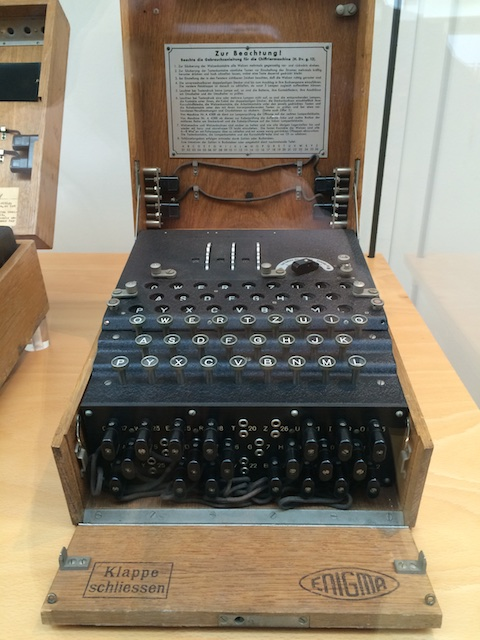
\includegraphics[scale=0.3]{enigmaFrankfurt.jpg}
\caption{An Enigma on display at the \textit{Museum f\"ur Kommunikation Frankfurt} \url{http://www.mfk-frankfurt.de}}
\end{marginfigure}

We eliminate $G$ by inserting $VW$ into the first equation, $WX$ into the second etc:

\begin{equation} \label{sixEnigma5}
\begin{split}
U V &= N^{-1} \sigma^{-1} N V W N \sigma N \\
V W &= N^{-1} \sigma^{-1} N W X N \sigma N \\
W X &= N^{-1} \sigma^{-1} N X Y N \sigma N \\
X Y &= N^{-1} \sigma^{-1} N Y Z N \sigma N
\end{split}
\end{equation}

We define the new unknown $H = N^{-1} \sigma^{-1} N$ and get

\begin{equation} \label{sixEnigma6}
\begin{split}
U V &= H (V W) H^{-1} \\
V W &= H (W X) H^{-1} \\
W X &= H (X Y) H^{-1} \\
X Y &= H (Y Z) H^{-1}
\end{split}
\end{equation}

So $UV$, $VW$ etc are conjugated by $H$. Each of the four equations in \ref{sixEnigma6} usually yielded several dozen solutions for $H$ and usually there is only one common solution to all four equations. This gave the code breakers $H$ and thus $N$, the internal wiring of the right rotor. The second rotor was cracked the same way because the German Nazis switched rotor positions every 3 months\footnote{It is amazing how little things in cryptography can trip up security of a system and open the doors to attackers. The German Nazis no doubt believed that by switching rotors they would increase the number of possible permutations (correct) and thus increase the security of their system (incorrect).} and a new rotor slid into the rightmost position. Rejewski and his team had daily keys for two months which happened to overlap with one rotor switching. They didn't have daily keys for a longer period that would span two rotor switchings, so they couldn't use this method to deduce the wiring of the third rotor. It's not clear how Rejewski and his colleagues cracked the wiring of the third rotor and the wiring of the reflector\footnote{For more details and possible solutions, see \bibentry{Vabek2006} \url{http://citeseerx.ist.psu.edu/viewdoc/summary?doi=10.1.1.186.9963&rank=1}.}, but they did. Using only two months worth of daily keys and intercepted messages the Polish cryptologists were able to deduce the internal wirings of the rotors of the Enigma Machine and with that were able to build a functioning replica of it. This achievement jumpstarted the effort of the British team at Bletchley Park and eventually resulted in the capability of the Allied Forces to listen in on all the transmissions encrypted with Enigma.







